\chapter{The modelled system}
\label{chap:qdots}
In this thesis, we apply our many-body methods to quantum dots, which are electrons confined in a potential. In accordance to popular manufacturing techniques, we use the common model of a two-dimensional parabolic quantum dot,  where $N$ electrons are confined in an isotropic harmonic oscillator potential in two spatial dimensions.\\
 This chapter serves to set up the mathematical framework for the description of those quantum dots, which is needed for all following calculations.

\section{The model Hamiltonian}
\label{sec:ModHam}
As discussed in the previous chapter, we can express the Hamiltonian as sum of a non-interacting and an interacting part. The non-interacting part is given as sum of the single-particle Hamiltonians $\hat{h}^{(0)}$, 
\be
\hat{H}_0 = \sum_i \hat{h}^{(0)}_i = \sum_i \lb -\frac{\hbar^2}{2m}\nabla_i^2 + \hat{v}_{i} \rb,
\label{eq:ho}
\ee
and composed of a kinetic and a potential part. 

\subsection{Harmonic oscillator basis}
In our case, the external potential is a harmonic oscillator one, which reads in two dimensions
\be 
\hat{v} = \frac{1}{2} m \omega^2 \rv^2 = \frac{1}{2}m\omega^2 (x^2+y^2).
\label{eq:potential}
\ee
As derived in chapter \ref{chap:theory}, the eigenfunctions of 
$\hat{h}^{(0)}$, specified by
\[
\hat{h}^{(0)}\phi_n = \epsilon_n \phi_n,
\]
are given as product of the one-dimensional solution in each dimension, 
\[\phi_n = \phi_{n_x,n_y} = \phi_{n_x}\phi_{n_y}.
\]
 Inserting for both factors the expression derived in Eq. (\ref{eq:HOsol}), we obtain
\be 
\phi_{n_x,n_y}(x,y) =  \sqrt{\frac{m\omega}{\pi\hbar}}(2^{(n_x+n_y)}n_x!\;n_y!)^{-\frac{1}{2}} H_n \lb \frac{m\omega}{\hbar x}\rb H_n \lb \frac{m\omega}{\hbar y} \rb e^{-\frac{m\omega}{2\hbar}(x^2 + y^2)},
\label{eq:SPCart}
\ee
where $H_n$ denotes the $n$th Hermite polynomial. The corresponding eigenvalues have been derived in chapter \ref{chap:theory}, too,
\be 
\epsilon_n = \epsilon_{n_x,n_y} = \hbar\omega (n_x+n_y+1).
\ee
Since the single-particle Hamiltonians $\hat{h}^{(0)}$ are invariant under orthogonal transformations, their eigenvalues do not depend on the chosen spatial coordinates. Considering that our chosen oscillator potential is spherically symmetric, i.e. the oscillator frequency $\omega$ is the same for both $x$- and $y$-dimension, it is common to express the single-particle orbitals in polar coordinates, instead of the Cartesian representation in Eq.~(\ref{eq:SPCart}). \\
For $d=2$ dimensions, one obtains the so-called \textit{Fock-Darwin orbitals} \cite{PhysRevB.80.045321},
\be 
\phi_{n,m_l}(r,\theta) = \sqrt{\frac{2n!}{(n+|m_l|)!}} \frac{e^{im_l\theta}}{\sqrt{2\pi}} L_n^{|m_l|}(r^2) e^{-r^2/2},
\label{eq:Laguerre}
\ee
where $n$ is the nodal quantum number ($n=0,1,2,\dots$) , and equals the number of nodes in the radial part,  $m_l$ is the orbital angular momentum quantum number ($m_l= 0,\pm 1, \pm 2, \dots$), and $L_n^{|m_l|}(x)$ are the generalized Laguerre polynomials. These ones are related to Laguerre polynomials as follows:
\be 
L^p_{q-p}(x) = (-1)^p \frac{d^p}{dx^p}L_q(x),
\ee
where the latter ones are polynomial sequences, defined as
\be 
L_q(x) = e^x \frac{d^q}{dx^q} \lb e^{-x} x^q \rb.
\ee
For further properties, we refer to \cite{liboff1992introductory,griffiths2005introduction}.
The Fock-Darwin orbitals are by construction eigenfunctions of the angular-momentum operator $L_z = -i\frac{\partial}{\partial\theta}$ with eigenvalue $m_l$. This gives the advantage of  having a basis that is diagonal in angular momentum. With quantum numbers $n,m_l$ instead of $n_x,n_y$, the eigenvalues of the single-particle Hamiltonians are given by
\be 
\epsilon_{n,m_l} = \hbar\omega(2n + |m_l| + 1).
\label{eq:emn}
\ee
Since the single-particle orbitals $\phi_{n,m_l}$ are denumerable, we can choose an ordering and identify each orbital with an integer. Recalling from Eq. (\ref{eq:SPspin}) that each single-particle state is modelled as product of spatial and spin part, we take into account that each orbit $\phi_{n,m_l}$ can be occupied by two particles, and specify the first one to have spin up, $m_s = +\frac{1}{2}$, and the second one to have spin down, $m_s = -\frac{1}{2}$. With this convention, our single-particle states can be labelled as shown in figure \ref{fig:shellstructure}.

\begin{figure}
\begin{center}
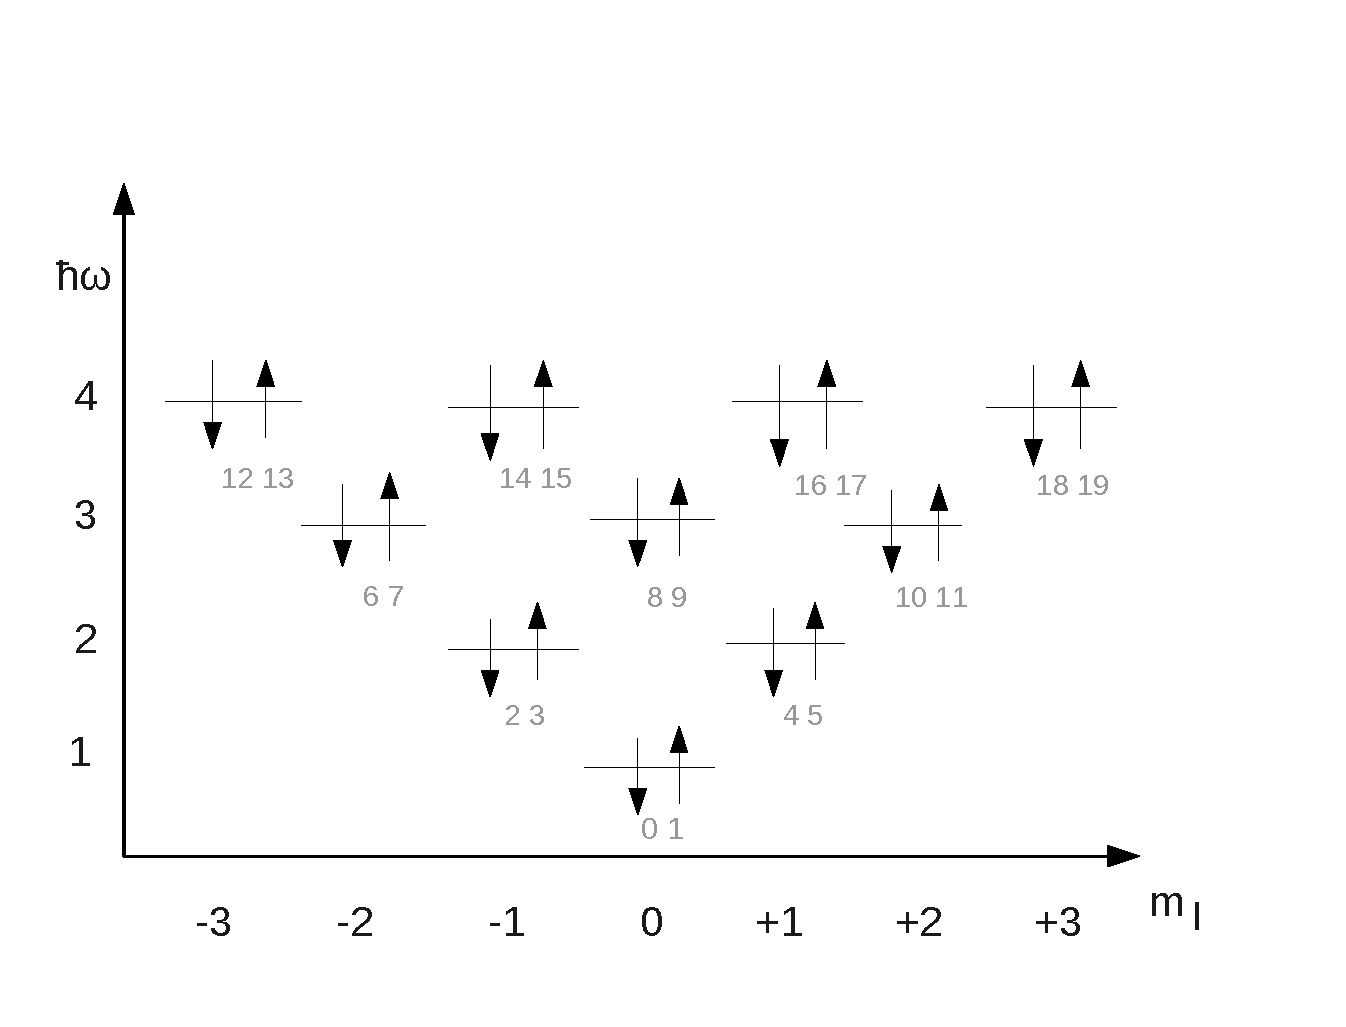
\includegraphics[scale=0.5]{../Plots/shellstructure1.pdf}
\end{center}
\caption{Labelling of the single-particle states of the two-dimensional harmonic oscillator. The $x$-axis shows the angular momentum quantum number, the $y$-axis the energy in units of $\hbar\omega$. Each energy level defines a shell $R$, with degenerate eigenvalues $\epsilon_i$ for the corresponding single-particle states. This arrangement is also referred to as \textit{shell structure}. }
\label{fig:shellstructure}
\end{figure}

\begin{table}
\begin{center}
\begin{tabular}[htb]{c c c}
\hline
$R$ & Degeneracy & Shell filling\\
\hline 
1 & 2 & 2 \\
2 & 4 & 6 \\
3 & 6 & 12 \\
4 & 8 & 20 \\
5 & 10 & 30 \\
\hline
\end{tabular}
\caption{Degeneracy for the first 5 shells and number of particles it takes to have a closed-shell system up to this level.}
\label{tab:shell}
\end{center}
\end{table}

Each index $i$ defines a specific set of quantum numbers $\lbrace n,m_l,m_s\rbrace$, where the relation between energy and quantum numbers $n$ and $m_l$ is determined by Eq. (\ref{eq:emn}). All eigenfunctions with same energy span a single-particle \textit{shell}. We define the shell number $R$ as\footnote{Note that another common convention is to define the shell number as $R=2n + |m_l|$. However, to directly compare our results with other current and previous master's students, studying our system with different many-body methods, we use the definition used in those theses.}
\be 
R = 2n + |m_l| + 1.
\ee
Each shell corresponds to an energy $\hbar\omega R$, and the degeneracy of each shell is given by $2R$, where the factor of $2$ accounts for spin.  If all single-particle states up to a certain shell are occupied, one has so-called \textit{closed-shell systems}.\\
These are the systems  we will consider in this thesis, suggesting that our number of particles is  restricted to $2,6,12,20,\dots$ The outstanding feature of closed-shell systems is their symmetry, since none of the degenerate energy levels is in a way more or less preferred.

To choose the eigenfunctions of the single-particle Hamiltonian as basis is a natural starting point with respect to the underlying physics, since the interaction can be considered as perturbation from the non.interacting case. Moreover, the basis allows an easy symmetrization of the many-fermion wave function and results in a fast convergence of the ground state energy as function of the basis size \cite{rontani:124102}.

\subsection{Choice of interaction}
Having $N$ electrons trapped in a two-dimensional isotropic harmonic oscillator potential, it is necessary to specify the type of interaction. In our case, we choose a two-body Coulomb potential,
\[
v(r_{ij}) = \frac{e^2}{4\pi\epsilon_0\epsilon_r}\frac{1}{r_{ij}},
\]
where $r_{ij} = \Vert \rv_i - \rv_j \Vert$ denotes the distance between two particles, $e$ the electron charge, $\epsilon_0$ the vacuum permittivity, and $\epsilon_r$ the relative permittivity.  Note that for the remainder of this thesis, we will use atomic units, setting $\hbar = m = e = 1/4\pi\epsilon_0 = 1$. Thus the energy is given in Hartrees,
\be 
E_H = \frac{m_e e^4}{(4\pi\epsilon_0\hbar)^2} = 4.35974418\times 10^{-18}J.
\ee 
This system of natural units is especially convenient for atomic physics calculations. On the one hand, it simplifies the equations, on the other hand it avoids orders of magnitude that give rise to numerical truncation and round-off errors.
In these units, the total Hamiltonian is  given by
\begin{align}
\hat H &= \hat H_0 + \hat H_I \notag \\
&= \sum_{i=1}^N \left(-\frac{1}{2}\nabla_i^2 + \frac{1}{2} \omega^2r_i^2\right) + \sum_{i<j} \frac{1}{r_{ij}}.
\label{eq:QDotH}
\end{align}


\section{Model space}
The basis functions for the $N$-particle Hilbert space are Slater determinants, as defined in \mbox{Eq. (\ref{eq:SDeterminant})}. Since there in principle exist infinitely many single-particle states  for the $N$ particles to occupy, the number of possible Slater determinants is infinite, too. For numerical calculations, one therefore uses a finite-dimensional subspace $\mathcal{P}\subset \mathcal{H}$ of the full Hilbert space, called \textit{model space}. The model space has a basis $\mathcal{B}$ with a finite number of Slater determinants, and its orthogonal projector is given by
\be 
P = \sum_{|\Phi_b\rangle \in \mathcal{B}} |\Phi_b\rangle\langle\Phi_b|.
\ee
In practice, one truncates the number of included single-particle states by specifying a maximal shell number $R$, such that the $N$ particles can maximally occupy $n= R(R+1)$ states:
\be 
\mathcal{B} = \mathcal{B}_R = \left\lbrace |\Phi_b\rangle : \max_{i=1\dots N} R_i \leq R \right\rbrace,
\ee
where $R$ is called energy-cut\footnote{Another common practice is to cut the global shell number instead of the single-particle shell number, \mbox{$\mathcal{B}_R = \left\lbrace |\Phi_b\rangle : \sum_{i=1}^N R_i \leq R \right\rbrace$}, see \cite{PhysRevB.80.045321}.}. As $R\rightarrow\infty$, the whole Hilbert space is spanned, such that the eigenvalues of $P\hat{H}P$ converge to the ones of $\hat{H}$. 

\section{Symmetries of $\hat{H}$}
Our Hamiltonian exhibits several symmetries, making it possible to reduce the complexity of the computations.  First of all, we have that 
\be 
[\hat{H},\hat{L}_z] = [\hat{H},\hat{S}_z] = 0.
\label{eq:commut}
\ee 
Here $\hat{L}_z$ is the angular momentum operator with eigenvalue\footnote{Since we are now using dimensionless units and not dealing with masses $m$ any more, we use the common notation $m_l\rightarrow m$ for the azimuthal quantum number.} $M = \sum_{i=1}^N m_{i}$,
\be 
\sum_{i=1}^N \hat{L}_z(i)|\Phi\rangle = M|\Phi\rangle.
\ee
The spin projection operator $\hat{S}_z$ is given by
\be 
S_z = \frac{1}{2}\sum_{p,\sigma} \sigma \ad_{p,\sigma} a_{p,\sigma},
\ee
with eigenvalues $M_s = \sum_{i=1}^N \sigma_i/2$. Since the Slater determinants are eigenvectors of both $\hat{L}_z$ and $\hat{S}_z$, our model space $\mathcal{P}$ is naturally split into subspaces with constant angular momentum $M$ and spin projection $M_s$. In other words, the Hamiltonian is block-diagonal in $M$ and $M_s$, such that a diagonalization of $\hat{H}$ can be done within each block separately. In particular, when interested in the ground state energy only, it is sufficient to set up the block with $M=M_S = 0$ and diagonalize that one, which reduces the computational effort enormously.

In principle, the matrix blocks could be even smaller, since our
 Hamiltonian (\ref{eq:QDotH}) also commutes with the total spin $\hat{S}^2$, given by
\be 
 \hat{S}^2 = \hat{S}_z^2 + \frac{1}{2}(\hat{S}_+ \hat{S}_{-} + \hat{S}_{-}\hat{S}_+),
\ee
where the spin raising and lowering operators are
\be 
S_{\pm} = \hat{S}_x \pm i \hat{S}_y = \sum_p \ad_{p\pm} a_{p \mp}. 
\ee
However, since the Slater determinants are not eigenfunctions of $\hat{S}^2$,  we would have to take a linear combination of them to obtain this property \cite{rontani:124102}. Therefore we restrict us to identities (\ref{eq:commut}).


